% KSe.tex
% $Author$ $Date$

% Predrag                   jun 20 2006
% Vaggelis                  may 20 2006

\section{\KSe}
\label{s-KS}
% Predrag                    4jul2006
% extracted from ~dasbuch/book/chapter/PDEs.tex  5jun2005 version
% Predrag                   17sep1999

% \PC{incorporate missing refs from chapter/refsPDEs.tex}

The \KS\ [KS] system\rf{ku,siv}, which arises in the description of
stability of flame fronts, reaction-diffusion systems and many other
physical settings, is one of the simplest nonlinear PDEs that
exhibit spatiotemporally chaotic behavior. In the formulation
adopted here, the time evolution of the ``flame front velocity''
$u=u(x,t)$ on a periodic domain $u(x,t) = u(x+L,t)$ is given by
\beq
\PCedit{
  u_t+{\textstyle\frac{1}{2}}(u^2)_x+u_{xx}+ u_{xxxx}=0
       }
% abandoned the CCP convention: u_t=(u^2)_x-u_{xx}- u_{xxxx}
    \,,\qquad   x \in [0,L]
    \,.
\ee{ks}
Here $t \geq 0$ is the time, and
$x$ is the spatial coordinate.
The subscripts $x$ and $t$ denote partial derivatives with respect to
$x$ and $t$. In what follows we use interchangeably the ``dimensionless
system size'' $\tildeL$, or the periodic domain size $L= 2\pi \tildeL$,
as the system parameter.

Spatial periodic boundary condition $u(x,t)=u(x+L,t)$
makes it convenient to work in the Fourier space,
\beq
  u(x,t)=\sum_{k=-\infty}^{+\infty} a_k (t) e^{ i k x /\tildeL }
\,,
% \label{fseries}
\ee{eq:ksexp}
%where $\tildeL=L/2\pi$. Thus,
with the $1$-dimensional PDE \refeq{ks}
replaced by an infinite set of
ODEs for the complex Fourier coefficients $a_k(t)$:
\beq
\dot{a}_k= \pVeloc_k(a)
     = ( (k/\tildeL)^2 - ( k/\tildeL)^4 )\, a_k
\PCedit{
    - i \frac{k}{2\tildeL} \sum_{m=-\infty}^{+\infty} a_m a_{k-m}
       }
\,.
\ee{expan}
Since $u(x,t)$ is real,
$ %\[
a_k=a_{-k}^*
\,,
$ %\] %\label{cplx-b}
and we can replace the sum in \refeq{expan} by a
sum over $k > 0$.

\PC{this text to be moved to a more appropriate place}
Due to the hyperviscous damping
$u_{xxxx}$, long time solutions of \KSe\ are smooth,
$a_k$ drop off fast\PC{how fast?} with $k$, and truncations
of \refeq{expan} to $N$ terms, $16 \leq N \leq 128$, yield
highly accurate solutions for system sizes considered here.
Robustness of the Fourier representation of KS as
a function of the number of modes kept in truncations
of \refeq{expan} is, however, a subtle issue.
Adding an extra mode to a truncation of the system
introduces a small
perturbation. However, this can (and often will)
throw the dynamics into a different asymptotic state.
A  chaotic attractor for $N=15$ can collapse into
an attractive period-3
cycle for $N=16$, and so on.
If we compute, for example, the Lyapunov exponent
$\Lyap(\tildeL,N)$ for a strange attractor of the
system \refeq{expan}, there is no reason to
expect $\Lyap(\tildeL,N)$ to smoothly converge to a limit
value $\Lyap(\tildeL,\infty)$ as $N \rightarrow \infty$,
because of the lack of structural stability both
as a function of truncation $N$, and the system size \tildeL.
The topology is more robust for \tildeL\ windows of transient turbulence,
where the system can be structurally stable,
and it makes sense to compute
 Lyapunov exponents, escape rates, etc., for the
{repeller}, \ie, the closure of the set of all
{unstable} periodic orbits.

Spatial representations of
PDEs (such as the 3$d$
snapshots of velocity and vorticity fields in Navier-Stokes)
offer little insight into detailed dynamics of low-$Re$ flows.
Much more illuminating are the \statesp\ representations.
\PC{expand this into a visualization subsection: how we use
    $d$-dimensional vectors (stability eigenvectors, etc) to project
    from $d$-dimensions to 2 or 3 dimensions. \underline{Not}
    Fourier modes as coordinates!}

The objects explored in this paper: \eqva\ and short \po s,
are robust both under mode truncations and small
system parameter $\tildeL$ changes.

%\PC{please generate and insert here a space-time plot of a
%    typical large \tildeL\ turbulent solution, with $\sqrt{2}$
%    basic wavelength in \tildeL units indicated, as in my seminar
%    presentations.
%   }

%%%%%%%%%%%%%%%%%%%%%%%%%%%%%%%%%%%%%%%%%%%%%%%%%%%%%%%%%%%%%%%%
\begin{figure}[t] \label{f:ks_largeL}
\begin{center}
\includegraphics[width=0.8\textwidth]{figs/ks_largeL.eps}
\end{center}
\caption{
A typical turbulent solution of the \KSe, system size
$L=8.886$.  The $x$
coordinate is scaled with the most unstable wavelength
$2\pi\sqrt{2}$, 
which is approximately also the mean wavelength of the turbulent flow. 
     }
\end{figure}
%%%%%%%%%%%%%%%%%%%%%%%%%%%%%%%%%%%%%%%%%%%%%%%%%%%%%%%%%%%%%%%%%%


\subsection{\Eqva\ and \reqva} % of the \KSe}
\label{sec:stks}
% former equilibria.tex

% Predrag                   jun 20 2006
% Vaggelis                  may 20 2006
% Predrag                                       05dec2004
% Lan                                           25nov2004
% from Lan thesis                                8jun2004

\Eqva\  (or the steady solutions)
are the simplest invariant sets in
the \statesp. 
\beq
 u(x,t) = u(x) %\,,\quad t \in \mathbb{R}
\,.
\ee{eqva}
More generally, due to the translational symmetry,
the KS system allows for \reqv\ solutions
(traveling waves, rotating waves),
characterized by a fixed profile $u_q$
moving with constant speed $c$, {\ie}
\beq
 u(x,t) =  u(x-ct) %\,,\quad t \in \mathbb{R}
\,.
\ee{reqva}
Because of the reflection symmetry (see \refsect{sec:KSeSymm}),
the \reqva\ come in pairs,
related by: $u(x) \to -u(-x)$, $c \to -c$.
\Eqva,  and
the connections between them form the
coarsest geometrical framework for organizing
\statesp\ orbits. %\rf{ksgreene88}.


In the Fourier space the \reqva\ are defined by the condition
\beq
 a_k(t) e^{-itc k/\tildeL} = a_k(0)
\,.
\ee{reqvaF}
Differentiating this condition with respect to time, we obtain
the \reqv\ condition,
\beq
 \pVeloc_k(a) - i \frac{k c}{\tildeL} a_k = 0
\,,
\ee{reqvCondF}
which needs to be solved for (time independent) $a_k$ and $c$.
\PC{\PCedit{replot \reffig{f:eqvSpatial} with new $u$ scale,
   and publication quality labels on axes.
    }}

%%%%%%%%%%%%%%%%%%%%%%%%%%%%%%%%%%%%%%%%%%%%%%%%%%%%%%%%%%%%%%%%
\begin{figure}[t] \label{f:eqvSpatial}
\begin{center}
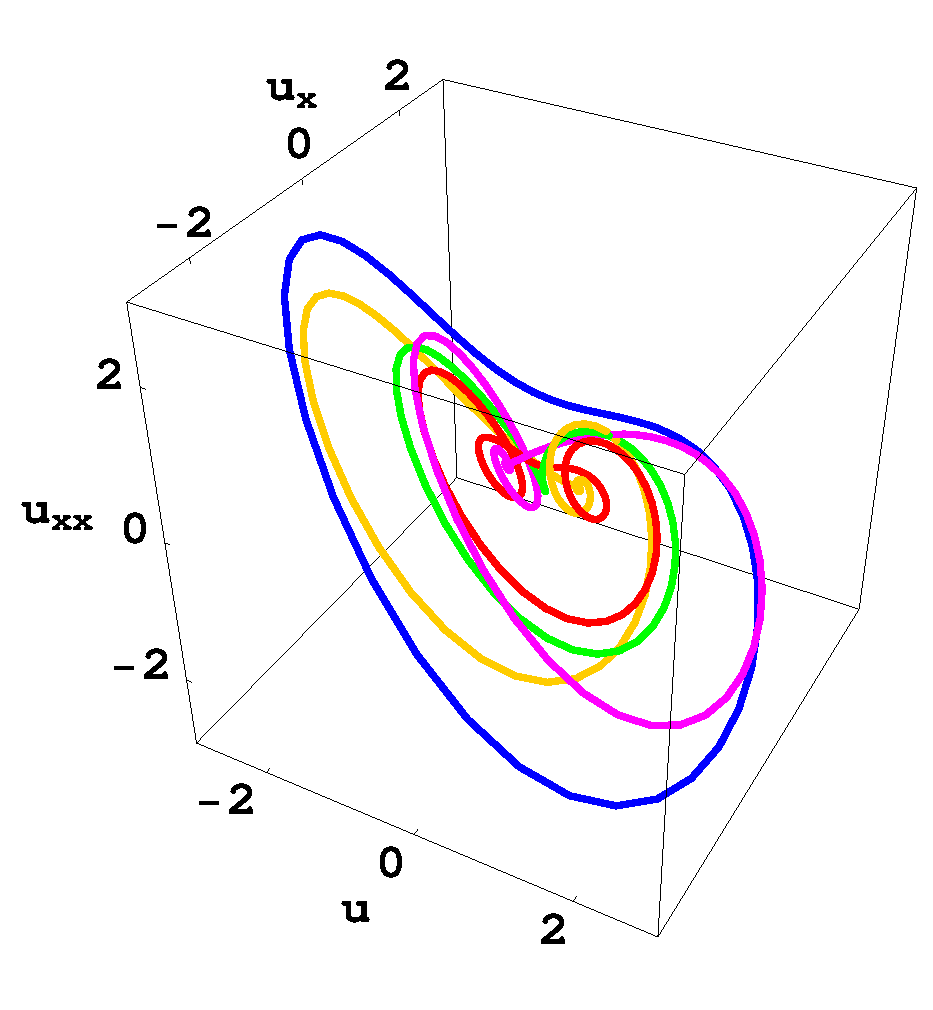
\includegraphics[width=0.4\textwidth]{figs/equilSpatial.eps}
\end{center}
\caption{
$(u,u_x,u_{xx})$ representation
of (blue) \EQV{1}, (red) \EQV{2},  (black) \EQV{3} \eqva,
 and (purple) \REQV{+}{1}, (orange) \REQV{-}{1} \reqva\ for
system size $L=22$. 
%, $N=64$ complex modes truncation.
        }
\end{figure}
%%%%%%%%%%%%%%%%%%%%%%%%%%%%%%%%%%%%%%%%%%%%%%%%%%%%%%%%%%%%%%%%%%

The \eqv\ condition $u_t=0$ for the {\KSe} PDE \refeq{ks}
is the ODE
\beq
{\textstyle\frac{1}{2}}(u^2)_x+u_{xx}+ u_{xxxx}=c \, u_x
% \,.
\ee{KSeqvCond}
which can be analyzed as a dynamical system in its own right.
Integrating once we get
\beq
{\textstyle\frac{1}{2}}(u-c)^2+u_x+u_{xxx}=\expctE
\,.
\label{eq:stdks}
\eeq
The integration constant \expctE\ can be interpreted as `energy',
see \refsect{sec:energy}.
Integrate over $L$, and $u_x$, $u_{xx}$ drop put by the
$L$ periodicity.
Written as a 3-dimen\-si\-on\-al dynamical system
with spatial coordinate $x$ playing the role of ``time'',
%\refeq{eq:stdks}
this is a volume preserving flow
\beq
u_x = v \,,\qquad
v_x = w \,,\qquad
w_x = - {\textstyle\frac{1}{2}}u^2-v+\expctE \,,
  \label{eq:3dks}
\eeq
with the ``time'' reversal symmetry,
\[
x \to -x,\quad u \to -u, \quad v \to v, \quad w \to -w \,.
\]
 Rewriting \refeq{eq:3dks} as
\beq
(u+w)_x=-{\textstyle\frac{1}{2}}u^2+\expctE
    =-{\textstyle\frac{1}{2}}(u-\sqrt{2\expctE}) (u+\sqrt{2\expctE})
\ee{eqvOfEqv}
we see that
for $\expctE<0$, $u+w$ increases without bound with $x \to \infty$,
and every solution escapes to infinity.
If $\expctE=0$, the origin $(0,0,0)$ is the
only bounded  solution, a marginally stable center with
eigenvalues $(0, i,-i)$.

For $\expctE>0$ there is rich
$\expctE$-dependent dynamics, with
fractal sets of bounded solutions investigated in
depth by Michelson\rf{Mks86}.
The solutions of the {\eqv}  condition
\refeq{eq:3dks} are themselves in turn  in turn organized by the
``{\eqva}  of {\eqva}''  condition
\( u_x= v_x= w_x= 0 \), and
the connections between them\rf{Mks86}.
    For $\expctE>0$ the {\eqv}  points of \refeq{eq:3dks} are
$c_{+}=(\sqrt{2\expctE},0,0)$ and $c_{-}=(-\sqrt{2\expctE},0,0)$.
Linearization of the flow around
$c_{+}$ yields the cubic equation
  \beq
\eigExp(1+\eigExp^2) = 4 \expctE
  \ee{KSeqvCubic}
for the
stability eigenvalues
$\eigExp[j] = \eigRe[j] \pm i \eigIm[j]$.
% of \refeq{KSeqvStab}.
They can
be given in any of the standard analytical forms for cubic
roots  (all useless in practice), such as
\beq
[ 2\eigRe \,, -\eigRe \pm i \eigIm ]
    \,,\qquad
\eigRe=\frac{1}{\sqrt{3}}\sinh \phi
\,,\qquad
\eigIm=\cosh \phi \, ,
\ee{eqvEqvEigV}
with $\phi$ fixed by $\sinh 3\phi=3\sqrt{6\expctE}$.
Hence $c_{+}$ has a {1\dmn}
unstable manifold and a 2\dmn\ stable manifold
along which solutions spiral in.
By the $x \to -x$ ``time reversal'' symmetry, the
invariant manifolds of $c_{-}$
have reversed stability properties.
Most orbits escape quickly even if initiated close to \eqva, and that
renders the numerical calculations
difficult\rf{ksham95,kshooper88,pimyk,pimsimp}.
In this context the variational method
developed in \refrefs{lanVar1,CvitLanCrete02}
appears more robust than
the earlier approaches.


%\subsection{\Eqva\ on a periodic domain}
%
For a periodic boundary cell of size
$L$ the only {\eqva}  are
solutions of \refeq{eq:3dks} of spatial periodicity $L$.
In the Fourier representation they satisfy
the \eqv\ condition for \refeq{expan}
% \PC{\rf{ksgreene88} to remarks}
\beq
( \frac{k^2}{\tildeL^2} - \frac{k^4}{\tildeL^4}  )\, a_k
    \PCedit{
    -  \frac{i k}{2\tildeL} \sum_{m=-\infty}^{+\infty} a_m a_{k-m}
            }
  = 0
\,.
\label{eq:stfks}
\eeq
Periods of spatially periodic {\eqva} are multiples of $L$.
Every time the system size crosses  $\tildeL=n$,
$n$-cell states
are generated through pitchfork bifurcations.
Due to the translational invariance of {\KSe},
they form invariant circles
in the full \statesp.
\PC{resurrect the commented text here}
% In the antisymmetric subspace considered here, they corresponds to two points,
% half-period translates of each other of the form
% \[
% u(x,t)=-2\sum_k b_{kn}\sin (knx) \,,
% \]
% where $b_{kn} \in \mathbb{R}$.
% % By rescaling $u,x$ and $\nu$, the $n$-cell states transform to each other.

For any fixed period $L$ the number
of spatially periodic solutions is finite up to a spatial translation.
For a sufficiently small $L$
the number of {\eqva} is small and
concentrated on the low wave-number end of the Fourier spectrum.

In a periodic box of size $L$
both \eqva\ and \reqva\ are  periodic solutions
embedded in 3-$d$ space \refeq{eq:3dks},
conveniently represented as loops in
$(u,v,w)$ space whose topology is controlled by the
``\eqva\ of \eqva'' stable-unstable manifold structure of
\refeq{eqvEqvEigV}, see \reffig{f:eqvSpatial}.
In this representation the continuous translation symmetry
is automatic - a rotation in the $[0,L]$ periodic domain only
moves the points along the loop. For an \eqv\ the points
are stationary in time; for \reqv\ they move in time, but in
either case, the loop remains invariant.
So we do not have the problem that we encounter in the Fourier
representation, where from the frame of one of the \eqva\
the rest trace out circles under the action of continuous symmetry
translations.

\noindent {\bf When is an \eqv\ important? a bit of speculation}
%
There are two kinds of roles
{\eqva} play:
(1)
a {\em ``hole'' in the natural measure}.
The more unstable eigendirections an \eqv\ has (for example, the
$u=$const \eqv~\EQV{0}), the more unlikely it is  that
an orbit will recur in its neighborhood.
(2)
{\em Unstable manifolds of the ``least unstable''{\eqva}}.
Empirically, asymptotic dynamics tends to spend
a large fraction of time in
neighborhoods of a few  {\eqva} with
a least number of unstable eigendirections.



\subsection{Symmetries of \KSe}
\label{sec:KSeSymm}
% former \subsection{Scaling and symmetries}
% former symm.tex
% Predrag extracted from newton.tex         jul  3 2006

The  KS equation is
Galilean invariant: if $u(x,t)$ is a solution, then
$u(x \PCedit{-ct,t) -c} $, with $c$ an arbitrary constant velocity, 
is also a solution.
Without loss of generality, in our calculations we shall set
the mean velocity of the  front to zero,
% \index{Galilean invariance}
% \index{invariance!Galilean}
\beq
\int dx \, u = 0
\,.
\ee{GalInv}
As  $\dot{a_0}=0$ in \refeq{expan},
$a_0$ is a conserved quantity, in our calculations
fixed to $a_0=0$ by the Galilean invariance condition \refeq{GalInv}.
The KS equation  \refeq{ks} is time translationally invariant,
and
space translationally invariant
under the 1-$d$ Lie group of $O(2)$ rotations: if
$u(x,t)$ is a solution, then $u(x+d,t)$ is an equivalent
solution for any $-L/2 < d \leq L/2$.
The KS equation is also invariant under
reflection (``parity'' or ``inversion'') operation
\beq
\Refl u(x) = -u(-x)
\ee{KSparity}
and the shift symmetry operation
\beq
\Shift u(x)=u(x+L/2)
\,.
\ee{KSshift}
In the Fourier modes decomposition  this
symmetry corresponds to invariance under
\refeq{FModInvSymm}.
\PC{forward reference to \refeq{FModInvSymm}.}
This shift symmetry is a particular case of the
above translational $O(2)$ invariance; more generally,
KS allows for solutions invariant under any rational shift by
$L/m$. Any \rpo\ with such rational shift is eventually periodic.
\Rpo s without a discrete symmetry have irrational shifts
$d$, and are not segments of a periodic solution.


Relations $\Refl^2=\Shift^2=1$
induce a linear decomposition of the space of solutions into 4 invariant
subspaces\rf{KNSks90} via projection operators
$\Refl_1=(\matId+\Refl)/2$,
$\Refl_2=(\matId-\Refl)/2$,
$\Shift_1=(\matId+\Shift)/2$, and
$\Shift_2=(\matId-\Shift)/2$. The nonlinear term $(u^2)_x$ in the KS equation
mixes these subspaces, leading,
according to \refref{KNSks90}, to four invariant subspaces
(labeled by the corresponding projection operators):
\begin{romannum} % SIAM itemize}

 \item[$R_1$:] The space of antisymmetric functions,
 \item[$S_1$:] The space of L/2 periodic functions,
 \item[$R_1 S_1$:] The intersection of the above two,
 \item[$L$:] The space of functions invariant under $x\mapsto L/2-x,\ u\mapsto -u$.

\end{romannum} %itemize}
%\ES{Using notation of \rf{KNSks90} here, not sure if it exists elsewere.}
The dynamics within the $R_1$ space of antisymmetric functions
was studied in \refref{Christiansen:97,Lan:Thesis,LanCvi07}.


\subsection{Antisymmetric subspace}
\label{s:AntisymmSubsp}

With the help of the
reflection \Refl\ and shift symmetry {\Shift}
operations
\refeq{KSparity},
\refeq{KSshift}
the  attractor ${\cal A}_{tot}$ can be decomposed into four pieces:
 ${\cal A}_{tot}={\cal A} \cup S {\cal A}  \cup \Theta {\cal A}
  \cup \Theta S {\cal A} $.

A decomposition
of the attractor into four disjoint sets
is usually not possible, since sometimes $ {\cal A}$ overlaps with
$\Theta S{\cal A} $ (in this case $\Theta  {\cal A}$ will also  overlap with
$S {\cal A} $).
In any case  the set $ {\cal A}$ can be taken as
the fundamental
domain of the Poincar{\'e} map, with $S  {\cal A} $,
$\Theta  {\cal A} $ and $\Theta S  {\cal A} $ its images under the
$S$ and $\Theta$ mappings.


% The Fourier coefficients $a_k$ are in general complex numbers.
% % of time $t$.
% We can
% isolate the antisymmetric subspace of the system \refeq{ks-L} by
% considering the case of $a_k$ pure imaginary, $a_k= i a_k$, where
% $a_k$ are real, with the evolution equations
% \beq
% % \dot{a}_k=(k^2- k^4)a_k - k \sum_{m=-\infty}^{\infty} a_m a_{k-m}
% \dot{a}_k = (k/L)^2\left( 1 - (k/L)^2  \right)a_k
%    - (k/L) \sum_{m=-\infty}^{+\infty} a_m a_{k-m}
% \,.
% \ee{expan-symm}

Since \KSe\ preserves
antisymmetric solutions, one can isolate the antisymmetric
subspace
$u(x,t)=-u(-x,t)$, or in terms of Fourier coefficients,
$a_{-k}= - a_k$.
For Fourier coefficients which respect the $x \to -x$ symmetry of
\KSe, see discussion in \refref{Christiansen:97},
and references therein.
In \refrefs{Christiansen:97,Lan:Thesis}
this option was used to eliminate
the continuous translational symmetry.

In the antisymmetric subspace the translational
invariance of the full system reduces
to the invariance under discrete
translation by half a spatial period $2\pi L$.
In the Fourier representation \refeq{expan},
this corresponds to invariance under
\beq
a_{2m} \to a_{2m}
    \,,\qquad
a_{2m+1} \to -a_{2m+1}
% \,, m \in \mathbb{Z}
\,.
\ee{FModInvSymm}
The antisymmetric condition amounts to imposing
$u(0,2\pi L)=0$ boundary condition, with
the size of the system reduced to
the $[0, \pi L]$ interval
\ES{Greene and Kim show that steady states (non-traveling)
have to be antisymmetric and our findings verify it.
Thus when discussing \eqva\ this conversion is not
meaningful.}.

In this paper we study the full \KS\ system invariant
under continuous translations. Due to the lack of self-adjointness
(non-normality) of the linearized \KS\ flow,
the antisymmetric subspace
is unstable under small perturbations and generic solution of
\KSe\ belongs to the full, periodic space. Nevertheless, some of
the \eqva\ and of the shortest periodic orbits lie in this subspace
and can play important role for the topology of the flow - examples
of such solutions will be discussed in \refsect{s:L22}.


\subsection{Stability of \eqva}
\label{s:StabEqui}
%%
% Predrag           5jun2005
% extracted from \Chapter{stability}{ 2apr2005}

If $u_\stagn(x)$ is an \eqv\ solution of \KSe,
the linear {\stabmat}
${\Mvar}={\Mvar}(a_\stagn)$
% , its matrix of its stability exponents
% in \refeq{die}
% local expansion rate
is constant in time,
and
the {\jacobianM}
of the \eqv\ solution is
\[
 \jMps^t(a_\stagn) = e^{{\Mvar} t}
    \,\qquad
 \Mvar_{ij}= \Mvar_{ij}(a_\stagn)
\,.
\]
The {\stabmat}
% \refeq{DerMatrix}
follows from \refeq{expan}:
% \index{Kuramoto-Sivashinsky system}
\beq
{\Mvar}_{kj}(a) % =\frac{\pde v_k(a)}{ \pde a_j  }
=((k/\tildeL)^2- (k/\tildeL)^4)\delta_{kj} \PCedit{+ (k/\tildeL)} a_{k-j}
\,.
\ee{expanMvar}
For the \KSe\ the constant solution $u(x,t)=0$ with zero energy $E$ is an
\eqv\ point of \refeq{ks} which we shall henceforth refer to as
\EQV{0}. For this ``laminar'' \eqv\ the {\stabmat}
is diagonal, and
so is the {\jacobianM}
$
\jMps^t_{kj}(0) = \delta_{kj} e^{((k/\tildeL)^2- (k/\tildeL)^4)t}
\,.
$

The $|k|<\tildeL$
long wavelength perturbations of the flat-front {\eqv}
are linearly unstable, while all
$|k|> \tildeL$ short wavelength perturbations are strongly contractive.
The high $k$ eigenvalues, corresponding to rapid variations of
the flame front, decay so fast that the corresponding eigendirections
are physically irrelevant.
% \index{Lyapunov exponent!{\eqv}}
To illustrate the rapid contraction in the non-leading eigendirections
we plot  in [MAYBE INCLUDE] % \reffig{f:eigenvalues}
the eigenvalues of the \eqv\ in the unstable regime,
for relatively small system size, % low viscosity $\nu$,
and compare them with the
stability eigenvalues of the least unstable cycle for the same
system size.
The ``laminar'' \EQV{0}~\eqv\ is very unstable,
with many unstable eigendirections.


From \refeq{expan} we see that the origin $u(x,t) = 0$
has Fourier modes as the  linear
stability eigenvectors.
For $0 \leq |k| \leq \tildeL$, these Fourier modes are
unstable.
The most unstable mode, nearest to $|k|=\tildeL/\sqrt{2}$,
sets the scale of the mean wavelength $\sqrt{2}$
of the spatiotemporal dynamics of the {\KSe},
measured in the system size \tildeL, see \reffig{f:ks_largeL}.


% The growth of the unstable long wavelengths (low $|k|$) excites
% the short wavelengths
% through the nonlinear term in \refeq{expan}.  The excitations thus
% transferred are dissipated by the strongly damped short wavelengths,
% and a ``chaotic \eqv\'' can emerge. The very short
% wavelengths $|k| \gg 1 / \sqrt{\nu}$ remain small for all times,
% but the intermediate wavelengths of order $|k| \sim 1 / \sqrt{\nu}$
% play an important role in maintaining the dynamical {\eqv}.
% As the damping parameter decreases, the solutions increasingly take on
% % Burgers type
% shock front
% character poorly represented by the Fourier basis, and many
% higher harmonics may need to be kept
% % \rf{KNS90,GEP}
% in truncations of
% \refeq{expan}.
%
%
% Hence, while one may truncate the high modes in the expansion
% \refeq{expan}, care has to be exercised to ensure that no modes
% essential to the dynamics are chopped away.

Even though our starting point
\refeq{ks}
is an infinite-dimensional dynamical system, the asymptotic dynamics
unfolds on a finite-dimensional attracting manifold, and so we are back on
the familiar territory of
%\refsect{SecDynFlows}:
the theory of a finite number of ODEs applies to this
infinite-dimensional PDE as well.

\subsection{Bifurcation structure of \KS}
\label{sec:KSlit}
% former KSlit.tex
%
% Vaggelis               jan 20 2007
% \subsection{\Eqva\ according to Greene and Kim}

Our study of the \eqva\ of
\KSe\ based on several classical papers in the field,
in particular the bifurcation and symmetry analysis of
Kevrekidis, Nicolaenko and Scovel\rf{KNSks90},
and
Greene and Kim\rf{ksgreene88}. What is new here is
a detailed exploration of the \eqva\ stable/unstable manifolds
for a specific system size $L = 22$, determination
of a large number of \rpo s, and a preliminary
exploration of the relation between the
observed spatiotemporal ``turbulent" patterns and
the \rpo s.


% What is the non-dimensional ``Rayleigh'' number for the
% \KS\ system?
%  Scaling out the ``viscosity'' $\nu$
% \[
% x \to x \nu^{\frac{1}{2}}
% \,,\quad
% t \to t \nu
% \,,\quad
% u \to u \nu^{-\frac{1}{2}}
% \,,
% \]
% brings the \KSe\ \refeq{ks}
% to a non-dimensional form
% \beq
% u_t=(u^2)_x-u_{xx}- u_{xxxx}
% \,,\qquad
%   x \in  [0,L\nu^{-\frac{1}{2}}] = [0,2\pi\tildeL]
% \,.
% \ee{ks-L}
% In this way the ``viscosity'' $\nu$
% and the system size $L$ are trade in for a single
% dimensionless system size parameter
% \beq
%   \tilde{L}={L}/{(2 \pi \sqrt{\nu})}
% % \tilde{L}=\frac{L}{2 \pi \sqrt{\nu}}
% % \,,
% \ee{tildeL}
% which plays the role of a ``Reynolds number''
% for the \KS\ system.

In the literature \refeq{ks} is sometimes written as
\beq
    u_t=(u^2)_x-u_{xx}- \nu \, u_{xxxx}
    \,,\qquad   x \in [0,L]
    \,,
\ee{ksVisc}
or in any number of other variants, all equivalent.
The \KSe\ in  form \refeq{ks} is used by
\cite{cross93,Mks86,ks04com}, for axample.
% \RLD{I've used the same convention as Kassam and Trefethen.
% If you google 'Kuramoto-Sivashinsky',
% http://mathworld.wolfram.com/Kuramoto-SivashinskyEquation.html is
% the first in the search list and it uses the same convention
% (actually, their $u$ is actually a $w$ such that $w_x$ is my $u$.)
% The site refers to a 1986 Physica D paper by Michelson and a
% "Handbook of differential equations" by Zwillinger, but I haven't
% seen either of these.  }
Here we use
$L$ as the system parameter, with the ``hyper-viscosity" $\nu$ fixed to $1$.
Other authors vary  $\nu$, with $L$ fixed to either $1$ or $2\pi$.
To minimize confusion,
in what follows we shall state results of all
calculations either in units of the dimensionless system size $\tildeL$,
or the systems size $L = 2 \pi \tildeL$. The parameter $\alpha$
of \refrefs{KNSks90,ksgreene88} is in this convention is
$\tildeL=\sqrt{\alpha/4}$.
    \PC{extend \reffig{fig:ksBifDiag} to $\tildeL=4$}


For small $\tildeL$ the only \eqv\ of the system is the
constant solution $y(x,t)=0$,
globally attracting
for $\tildeL<1$. At $\tildeL=N$, $N=1,2,3, \dots$,
the $N$th harmonic becomes unstable and the constant solution
undergoes a pitchfork bifurcation into
the antisymmetric ``$N$-cell'' states\rf{ksgreene88}.
These states contain only the multiples of the $N$th
harmonic, {\ie}, only non-vanishing Fourier coefficients
are $(a_N,a_{2N},\dots)$.
Greene and Kim show that symmetric solutions are \eqva, not \reqva.
    \PC{mark point $A$ in \reffig{fig:ksBifDiag}}
% At point $A$ in \reffig{fig:GreeneKim}
At point $A$ in \reffig{fig:ksBifDiag}
the $1$-cell state loses stability
and bifurcates to a stable,
asymmetric \reqv, which in turn becomes unstable
through a Hopf bifurcation at point $Z$.
        \PC{mark point $Z$ in \reffig{fig:ksBifDiag}}


At $\tildeL=2$ a $2$-cell \eqv\ bifurcates off the \EQV{0} \eqv.
% At point $B$ in \reffig{fig:GreeneKim}
At point $B$ in \reffig{fig:ksBifDiag}
the $1$-cell branch merges to the $2$-cell branch.
In general each $N$-cell branch merges to the corresponding $2N$-cell branch.

% At point $C$ in \reffig{fig:GreeneKim}
At point $C$ in \reffig{fig:ksBifDiag}
the $2$-cell state bifurcates to a type of
\eqv\ solution
found by La Quey, Mahajan, Rutherford and Tang\rf{laquey74} 
and generalized by Greene and Kim who refer to them as GLMRT \eqva.
For a GLMRT solution $u(x)$ is antisymmetric,
a long wavelength distorted $N$-cell state.

\PC{STUDY - this suggests that \expctE\ grows with system size:
   The last type of solution identified in \refref{ksgreene88}
   appears at point $F$  in reffig~{fig:GreeneKim} and is called a
 ``giant" state because its amplitude grows as the system size increases.
   }

According to the bifurcation diagram
% \reffig{fig:GreeneKim},
\reffig{fig:ksBifDiag}
and our numerical results,
at the system size $\tildeL=22/2\pi = 3.5014\dots$
studied here,
the {\eqva} are the $2$- and $3$-cell states \EQV{2} and \EQV{3},
the GLMRT \eqv\ that bifurcates from a $3$-cell state at point $I$
on \EQV{1},
the pair of \reqva\  \REQV{\pm}{1}
that belong to the branches starting at point
$A$,
and the ``$M$ branch"  \reqva\ \REQV{\pm}{2}.
\PC{\PCedit{replot \reffig{fig:ksBifDiag} with 
   (a) the new $u$ scale,
   (b) publication quality labels on axes 
   (c) continue {\eqva} that we use to $\tildeL=4$
   (d) \ESedit{Mark points C and M from \rf{ksgreene88} if
       are mentioned in text: the 2c to GLMRT bifurcation 
       and the GLMRT to \REQV{\pm}{2} bifurcation,
       points C and M.
       }
   (e) \tildeL range is $[1,4]$

    }}

%%%%%%%%%%%%%%%%%%%%%%%%%%%%%%%%%%%%%%%%%%%%%%%%%%%%%%%%%%%%%%%%
\begin{figure}[t]       \label{fig:ksBifDiag}
\begin{center}
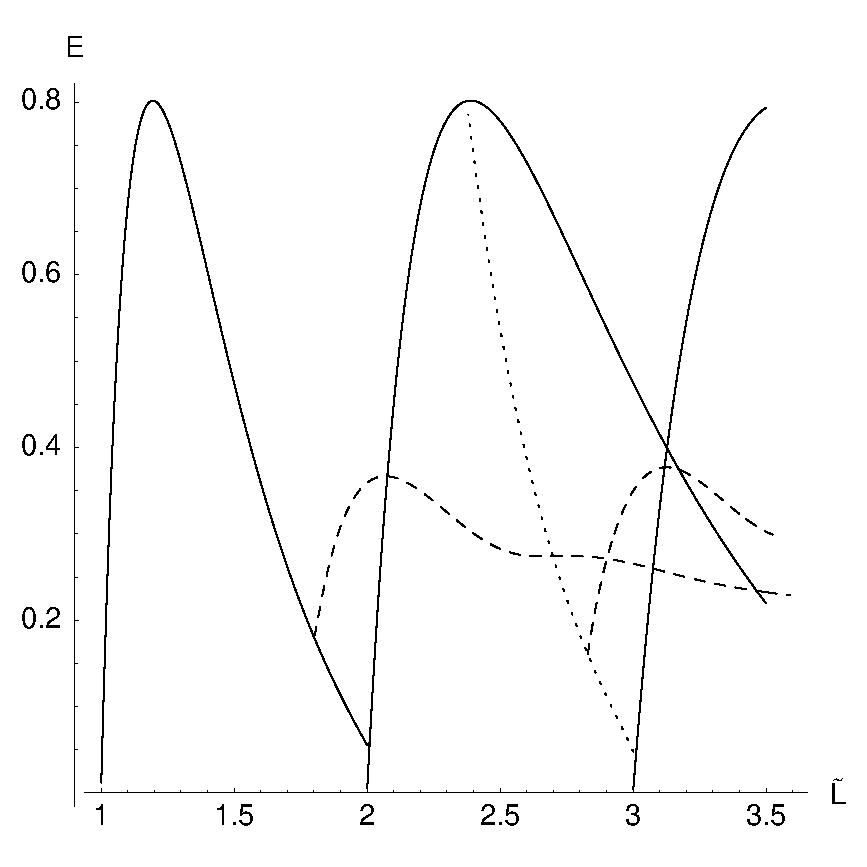
\includegraphics[width=0.5\textwidth]{figs/ksBifDiag.eps}
\end{center}
\caption{
The energy \refeq{ksEnergy}  of all  \eqva\ that exist up 
to $\tildeL = 3.5$
plotted as a function of the system size
$\tildeL$. 
Further \eqva\ not present at 
$\tildeL = 3.5$ are given in \refref{ksgreene88}).
Solid curves denote $n$-cell solutions,
dotted curves GLMRT, the dash-dotted curve the
`giant states', and dashed curves the \reqva.
Open circles indicate Hopf bifurcations.
The color of a branch indicates the number of unstable
eigenvalues: (red) 2 unstable eigenvalues, (blue) 1
unstable eigenvalue, (green) stable.
        }
\end{figure}
%%%%%%%%%%%%%%%%%%%%%%%%%%%%%%%%%%%%%%%%%%%%%%%%%%%%%%%%%%%%%%%%%%

        \PublicPrivate{%
        }{% switch to Private:

\subsection{Back in the saddle again}

Kevrekidis, Nicolaenko and Scovel~\rf{KNSks90}
prove that the bifurcation of the trivial state $y=0$ to an $N$-cell state is a pitchfork.
They observe that when the $1$-cell state losses stability at point $A$ the
eigenvector corresponding to the zero eigenvalue of the stability matrix aligns itself with the direction of uniform translation of the
system which, due to the translational invariance of \KSe\, also corresponds to a zero eigenvalue. Thus the algebraic multiplicity of the zero eigenvalue is $2$ while its geometric multiplicity is $1$. Using this fact and a local, $O(2)$-equivariant, approximation to the center manifold they prove that this type of bifurcation creates traveling waves.
        } %end \PublicPrivate{%

\section{\Rpo s}
% fromer history.tex
% Predrag created file              jul 3 2006

The KS equation  \refeq{ks} is time translationally invariant,
and
space translationally invariant
under the 1-$d$ Lie group of $O(2)$ rotations: if
$u(x,t)$ is a solution, then $u(x+d,t)$ is an equivalent
solution for any $-L/2 < d \leq L/2$.
As a result,
KS can have \reqva\ (traveling wave) solutions
$u(x-ct)$ and \rpo\ solutions with a nonzero shift
\beq
u(x+d,\period{}) = u(x,0)
\,,
\ee{KSrpos}
where $\period{}$ is the period.
\ES{Is this obvious to everybody? I cannot really see why it is so.}


{\Rpo s} were introduced by Poincar\'e in his study of
the 3-body problem\rf{ChencinerLink,rtb}.
\Reqva\ of this problem
are known as the Lagrange points. 
% They are stationary in
% the co-rotating frame, but
% in the inertial frame they execute circular motions.
{\Rpo s} are periodic orbits in appropriate co-rotating frame,
but in the inertial frame their trajectories
are quasiperiodic.
They arise in dynamics of physical systems
with continuous symmetries, such as motions of rigid bodies, gravitational
$N$-body problems, molecules and nonlinear waves.
For example, Viswanath\rf{ViswanathPC06} % arXiv.org/physics/0604062
has found both \reqva\ and \rpo s in the plane Couette problem.
Our initial searches for \rpo s in KS system were
inspired by Vanessa L{\'o}pez\rf{lop05rel} investigation
of {\Rpo s} of the Complex Ginzburg-Landau equation.
